\documentclass{article}

% if you need to pass options to natbib, use, e.g.:
%     \PassOptionsToPackage{numbers, compress}{natbib}
% before loading neurips_2020

% ready for submission
% \usepackage{neurips_2020}

% to compile a preprint version, e.g., for submission to arXiv, add add the
% [preprint] option:
%     \usepackage[preprint]{neurips_2020}

% to compile a camera-ready version, add the [final] option, e.g.:
%     \usepackage[final]{neurips_2020}

% to avoid loading the natbib package, add option nonatbib:
\usepackage{neurips_2020}
\usepackage[cache=false]{minted}
\usepackage[utf8]{inputenc} % allow utf-8 input
\usepackage[T1]{fontenc}    % use 8-bit T1 fonts
\usepackage{hyperref}       % hyperlinks
\usepackage{url}            % simple URL typesetting
\usepackage{booktabs}       % professional-quality tables
\usepackage{amsfonts}       % blackboard math symbols
\usepackage{nicefrac}       % compact symbols for 1/2, etc.
\usepackage{microtype}      % microtypography
\usepackage{amsmath}
\usepackage{wrapfig}

%\usepackage{newunicodechar}
%\usepackage{fontspec}
%\newfontface\mathsymbolfont{Latin Modern Math}
%\newunicodechar{ϕ}{{\mathsymbolfont\mitphi}}

\newenvironment{tab}[2][\linewidth]
{\begin{tabular*}{#1}[t]{@{\extracolsep{\fill}}>{\hspace{4pt}}#2}}%
{\end{tabular*}}

\usepackage{trimspaces}
\newcommand*{\trim}[1]{%
  \trim@spaces@noexp{#1}%
}
\usepackage{tikz}
\usetikzlibrary{decorations.pathreplacing,shapes,arrows,positioning,calc}

\tikzset{
  cfedge/.style={
    font=\itshape,
    draw=black,
    ->,
    >=stealth'
  },
  process/.style={
    draw,
    fill=orange!50,
    rectangle,
    minimum height=1.5em,
    minimum width=4em,
    align=center,
    font=\small,
  }
}

\newcommand{\todo}[1]{{\color{red} TODO: #1}}
\newcommand{\wmnote}[1]{{\color{blue} Billy: #1}}
\newcommand{\vcnote}[1]{{\color{yellow} Valentin: #1}}
\newcommand{\define}[1]{\textbf{\emph{#1}}}

\title{Instead of Rewriting Foreign Code for Machine Learning, Automatically Synthesize Fast Gradients}

\author{%
  David S.~Hippocampus\thanks{Use footnote for providing further information
    about author (webpage, alternative address)---\emph{not} for acknowledging
    funding agencies.} \\
  Department of Computer Science\\
  Cranberry-Lemon University\\
  Pittsburgh, PA 15213 \\
  \texttt{hippo@cs.cranberry-lemon.edu} \\
  % examples of more authors
  % \And
  % Coauthor \\
  % Affiliation \\
  % Address \\
  % \texttt{email} \\
}

\begin{document}

\maketitle


\begin{abstract}
Applying differential programming techniques and machine learning algorithms to foreign programs requires developers to either rewrite their code in a machine learning framework, or otherwise provide derivatives of the foreign code.
This paper presents Enzyme, a high-performance automatic differentiation (AD) compiler plugin for the LLVM compiler framework capable of synthesizing gradients of statically analyzable programs expressed in the LLVM intermediate representation (IR). Specifically, Enzyme can synthesize gradients for programs written in any language whose compiler targets LLVM IR including C, C++, Fortran, Julia, Rust, Swift, MLIR, etc., thereby providing native AD capabilities in these languages. Unlike traditional source-to-source and operator-overloading tools, Enzyme performs AD on optimized IR. On a machine-learning focused benchmark suite including Microsoft's ADBench, AD on optimized IR achieves a geometric mean speedup of 1.6x\todo{put real number} over AD on IR before optimization. Packaging Enzyme for PyTorch and Tensorflow provides convenient access to gradients of foreign code with state-of-the art performance, enabling foreign code to be directly incorporated into existing machine learning workflows. 
\end{abstract}

\section{Introduction}
\label{sec:intro}

Machine learning frameworks such as PyTorch\cite{paszke2017automatic} and Tensorflow\cite{abadi2016tensorflow} have become widespread as the primary workhorses of the modern machine learning community. In order to compute the necessary gradients for algorithms such as backpropagation\cite{hecht1992theory}, bayesian inference, and uncertainty quantification \cite{Wang2018-yr}, however, programmers are required to rewrite all of their code to be in said framework. This rewriting is especially problematic for applying machine learning to new domains as existing tools like physics simulators\cite{feng2016fastpm, broughton2020tensorflow, NIPS2018_7948, degrave2019differentiable, hu2019difftaichi}, game engines, climate models \cite{Stevens2020-ir}, and medical models\cite{alquraishi2019end} that are not written in the domain specific languages of machine learning frameworks. 
%Additionally, as the field of differential programming has become more mature, the desire for differentiation as a first class operation in programming languages has resulted in many new automatic differentiation frameworks \cite{maclaurin2015autograd,jax2018github,SwiftAutodiff,zygoteMlsys}.

This rewriting has been identified as a quintessential challenge of applying machine learning to scientific computing.

"Integrating Machine Learning within in situ Application Workflows. The growing data sizes
and complexity associated with scientific applications, increasing performance gap between com-
pute and I/O capabilities, and significant data management challenges and costs at extreme scales
have led to significant interest in and support for in situ and in-transit data processing [432]. As
ML techniques become an important part of scientific application workflows, scalable in situ and
in-transit formulations and implementations of these techniques are also increasingly important.
Such implementations present significant challenges at all levels, from algorithmic formulations
and programming abstractions suitable to online and in situ and in-transit execution to runtime
services to manage the control and data flow of the overall workflow. For example, integrating
current ML libraries, such as Theano [416] and Caffe [414], requires significant code changes to
scientific workflows and analysis applications." \cite{Baker2019-ty}



The need to compute efficient derivatives has become necessary across a diverse set of domains ranging from machine learning, scientific programming, and more. 

Uses in Neural ODEs\cite{chen2018neural}.

There are four things desired from an AD tool: generality (the ability to differentiate arbitrary programs), ease of use, speed (computing derivatives should be efficient), and correctness (producing the right answer). Moreover, broadly speaking, automatic differentiation tools can be separated into three categories.

\define{Operator-overloading} approaches take advantage existing functionality compute derivatives of functions alongside the original code. Examples of this include Adept\cite{adept}, which provides differentiable types in C++ that . These approaches require rewriting your source code to use the differentiable types/operation in place of standard language utilities, and can often be slow as they must store what operations are taking place in order to later differentiate.

\define{Source-rewriting} approaches analyze the source code of programs and emit new source code that computes the derivative of a function. Examples include Tapenade\cite{TapenadeRef13}, a framework which computes forward and backwards mode derivatives for C and Fortran programs; and Zygote\cite{zygoteArxiv,zygoteDP,zygoteMlsys}, a framework that dynamically creates derivative functions in Julia's JIT. Such tools can be more efficient than operator-overloading approaches as they can statically analyze the computation. They also tend to only work with programs in a specific language, sometimes even only a subset of programs in that language.
%require the whole source needed for derivatives to be available at compile time and not automatically generated, say in a JIT. Derivatives computed with such tools, however, are easy to debug as it is clear what computation they are performing.

Finally, \define{high-level differential programming frameworks} approaches provide a library or domain-specific language (DSL) for users to write differential programs in. Such approaches dynamically create derivative functions for use by programmers and often just-in-time (JIT) compile derivatives for performance. Examples of this include DiffTaichi\cite{hu2019difftaichi}, a DSL for physics simulations; Halide\cite{Li:2018:DPI}, a DSL for image processing; PyTorch\cite{paszke2017automatic}, 
and TensorFlow\cite{abadi2016tensorflow}, Python libraries for machine learning. Such approaches require rewriting programs to be compatible with the framework, and AutoGrad\cite{maclaurin2015autograd} and JaX\cite{jax2018github}, Python libraries for differentiating numpy-style programs, also fall into this category. Programmers hoping to use these tools must rewrite their code to be compatible with the desired framework, but are often rewarded with high-level or domain-specific optimizations.

\wmnote{Discuss major need for high performance AD in probabilistic programming such as \cite{cusumano2019gen} }

We present Enzyme, an efficient cross-platform compiler for automatic differentiation.  This paper makes the following contributions:
\begin{itemize}

\item Enzyme, a compiler plugin for LLVM that can synthesize high-performing gradients of statically analyzable code in LLVM IR, including IR generated by compiler frontends for C, C++, Fortran, Rust, etc.

\item PyTorch-Enzyme, a foreign-function interface for the PyTorch machine learning framework that allows programmers to use code written in LLVM-compiled languages in their machine-learning workflows, as well as a similar foreign-function interface for TensorFlow.

\item Enzyme.jl, a package that uses Enzyme to synthesize high-performing gradients of Julia code, which demonstrates that gradients of code written in a dynamic high-level language can be generated statically and perform well with only low-level information.

\item A study demonstrating that AD as part of the compilation process can outperform source-level tools on a standard machine learning benchmark suite~\cite{adBench} and achieve state-of-the-art performance.
\end{itemize}

There is therefore an unmet need of being able to take derivatives large hole of being able to provide 


%Embedding automatic differentiation as a first class citizen of the language, as is done in Swift\cite{SwiftAutodiff} arguably falls into this category.

\subsection{Related Work}

Clad is a plugin the the Clang compiler that implements forward and reverse mode automatic differentiation on a subset of C/C++ \cite{Vassilev_Clad}.
% tested on SmallPT raytracer and The ROOT Framework [15] is widely adopted in high-energy physics for data analysis. It offers
a wide range of mathematical tools for fitting and minimization. These tools use extensively
derivatives and some of them are hand-written while others are numerically calculated. We plan
on adopting Clad in ROOT6 through its C++ interpreter – Cling [13]

\subsection{Compilation and AD}
Performing derivatives before traditional optimizations have occurred, as in operator-overloading and source-rewriting tools, can result in asymptotically worse performance. Consider the example in Figure \ref{fig:licm}.

\begin{figure*}
    \centering
\begin{minted}[fontsize=\small]{c}
double mag(const double* x);//Compute magnitude in O(N)
void norm(double* out, double* in) {
    // double res = mag(in); code motion optimization can move outside the loop
    for(int i=0; i<N; i++) { out[i] = in[i]/mag(in); }
}
\end{minted}
\begin{tabular}{c|c}
\begin{minipage}[T]{0.49\linewidth}
\begin{minted}[fontsize=\small]{c}
// LICM, then AD, O(N)
void norm(double* out, double* dout,
         double* in, double* din) {
  double res = mag(in);
  for(int i=0; i<N; i++) {
    out[i] = in[i]/res;
  }
  double dres = 0;
  for(int i=0; i<N; i++) {
    dres += -in[i]*in[i]/mag * dout[i];
    din[i] += dout[i]/mag;
  }
  dmag(in, din, dres);
}
\end{minted}
\end{minipage}& \begin{minipage}[T]{0.49\linewidth}
\begin{minted}[fontsize=\small]{c}
// AD, then LICM O(N^2)
void norm(double* out, double* dout,
          double* in, double* din) {
  double res = mag(in, n);
  for(int i=0; i<n; i++) {
    out[i] = in[i]/res;
  }
  for(int i=0; i<n; i++) {
    double dres = -in[i]*in[i]/mag \
                        * dout[i];
    din[i] += dout[i]/mag;
    dmag(in, din, n, dres);
  }
}
\end{minted}
\end{minipage}
\end{tabular}
    \caption{In the second program, mag is still able to be moved outside as it is the same every iteration, however, dmag cannot be moved outside the loop as it reads/writes to the same memory.
}
    \label{fig:licm}
\end{figure*}

Analyses such as alias analysis\wmnote{cite} and use-def analysis traditionally found in the compiler are critical for efficient automatic differentiation. They are necessary building blocks for robust \define{activity analysis}, which aims to detect which instructions could impact the derivative computation and thus not need to compute adjoints for.





\begin{enumerate}
    \item Prior, rewrite legacy software in PyTorch/TensorFlow -- much work
    \item Manually define gradient (or use Tapendade + Adept slow and tedious)
    \item FFI that automatically creates gradient function
\end{enumerate}


%Being able to both integrate existing code and do so efficiently, Enzyme enables researchers to incorporate machine learning into an entirely new class of tools and application. 




% covid c rewrite https://twitter.com/neil_ferguson/status/1241835454707699713

"The key to making a scientific ML stack work is by making every component compatible with the AD-system. This is because, if there is just one part of your loss function that isn't AD-compatible, then the whole network won't train" \cite{10.15200/winn.156631.13064}



``[End-to-end] deep learning for [protein] structure prediction [has been difficult] stem[ming] from the technical challenge of developing an end-to-end differentiable model that rebuilds the entire structure prediction pipeline using differentiable primitives.'' \cite{alquraishi2019end}



By incorporating several compiler technologies, we also demonstrate 





* ML/Neurips:

People made their own dsl/implementation in Tensorflow. Don't have to do a 

* Systems story (AD story) how to do fused fwd/backwards optimizations how to do IR, type inference challenges, high level
 + sample codes, optimizations, benchmarks

* Differentiable programming crowd: cross-language AD [super cool in own right], integrating with legacy software

Differentiable programming in LLVM based languages



You don't have to write complicated losses in tensorflow math world:


Differentiating C/C++ [Fortran, Rust, XLA, etc]; 
fusing

\section{Design}
\label{sec:design}
Though it is clear that synthesizing gradients is better done after optimization, doing so requires working at a lower-level of abstraction which presents additional challenges.

Enzyme works in the following stages:
\begin{itemize}
    \item Analyze types and instruction activity
    \item For all active values, allocate and zero memory to create corresponding shadow values.
    \item For each Basicblock \texttt{B}, emit the adjoint for all instruction of \texttt{B} in reverse order
    \item Optimize
\end{itemize}


\AtBeginEnvironment{minted}{%
  \renewcommand{\fcolorbox}[4][]{#4}}



\newminted[codebox]{llvm}{texcl=true, autogobble=true,breaklines}

\begin{figure}
    \centering
\begin{tikzpicture}
\node[inner sep=0, outer sep=0] (orig) {
\begin{minipage}[T]{0.49\linewidth}
\begin{codebox}
define double @reluf(double %x)
entry:
  ; Shadow values for reverse
  ; alloca %d\_x = 0.0
  ; alloca %d\_call = 0.0
  ; alloca %d\_result = 0.0
  br (%x > 0), if.true, if.end
if.true:
  %call = f(%x)
  br cond.end
if.end:
  %res = phi[%call, if.true],      [0, entry]
  ret %res
\end{codebox}
\end{minipage}
};

\node[inner sep=0, outer sep=0, xshift=6.2cm] (reverse) {
\begin{minipage}[T]{0.49\linewidth}
\begin{minted}[fontsize=\small]{llvm}
reverse_if.end:
  ; adjoint of return
  store %d_result = 1.0
  ; adjoint of %result phi node
  %d_call += if %x > 0.0, (load %d_result), else 0
  store %d_result = 0.0
  br %cmp, %reverse_if.true, %reverse_entry
reverse_if.true:
  ; adjoint of %call
  %df = @diffe_f(%x)
  %d_x += %df * (load %call)
  store %d_call = 0.0
  br %reverse_entry
reverse_entry:
  %0 = load %d_x
  ret %0
\end{minted}
\end{minipage}
};
\end{tikzpicture}
    \caption{Example differential reverse creation for \texttt{relu(f(x))}. The left hand side shows the LLVM IR for the original computation, with commented out shadow allocations of active variables. The right hand side shows the reverse pass that Enzyme would generate to propagate gradient information across the program.}
    \label{fig:reluf}
\end{figure}

\begin{figure}
\centering
\begin{minted}[fontsize=\small]{c}
double sum(double* x) {
  double total = 0;
  for(int i=0; i<10; i++)
    total += read() * x[i];
  return total;
}

void diffe_sum(double* x, double* xp) {
  return __enzyme_autodiff(sum, x, xp);
}

void diffe_sum(double* x, double* xp) {
  double* read_cache = malloc(10*8);
  for(int i=0; i<10; i++)
    readCache[i] = read();
  // reverse
  for(int i=10-1; i>=0; i--)
    xp[i] += read_cache[i];
  }
  free(read_cache);
}
\end{minted}
\caption{Example of caching the result of read for the reverse pass and allocations for loops.}
\label{fig:cacheloop}
\end{figure}

\begin{figure}
\begin{minted}[fontsize=\small]{c}
double loadsq(double* x) {
  return x[0] * x[0];
}
void f(double* x) {
  *x = loadsq(x);
}

{double,double} augmented_loadsq(double* x) {
  return {/*return val*/x[0]*x[0], /*cache*/x[0] };
}

void diffe_loadsq(double* x, double* d_x, double d_ret, double cache) {
  d_x[0] += 2 * cache * d_ret;
}

void diffe_f(double* x, double* xp) {
  {call, cache} = augmented_loadsq(x);
  *x = call;
  double d_ret = *d_x;
  *d_x = 0;
  diffe_loadsq(x, d_x, d_ret, cache);
}
\end{minted}
\caption{Creating an augmented forward pass for a function to ensure requisite values are cached for the reverse.}
\label{fig:cacheaugment}
\end{figure}

\subsection{Shadow Memory}
For every active value in the original program, Enzyme creates and zero's a shadow version of that value. 

Local data structures with active variable need to be
duplicated to store derivative information
* Leverage all data structures are created by specific
memory instructions (malloc/free/new/delete/etc)
* Allocations are copied in forward pass to create
differential structures
* Frees are delayed until the reversed version of the
block that allocated in case values are used in the
reverse pass

\subsection{Type Analysis}

Types inside LLVM IR (and even C/C++) do not necessarily represent the type of the underlying data. For example, the \texttt{memcpy} function which copies data operates on generic pointers without types (\texttt{void*}). Creating a correct gradient for \texttt{memcpy}, however, requires knowing the type of the memory being copied. If you were copying 8 bytes of double data you would perform one double (8-byte) addition in the reverse pass, whereas if you were copying 8 bytes of float data you would need to do two float (4-byte) additions.

Taking the derivative of instructions such as \texttt{memcpy} depends on the type of the data being copied. As demonstrated in Figure \ref{fig:memcpy}, the derivative of a \texttt{memcpy} of memory containing doubles should add the propagate differential destination into the differential source, whereas a \texttt{memcpy} of pointer data should copy the differential source pointers into the differential destination in the forward pass, with nothing in the reverse. As these two operations are incompatible with each other (resulting in garbage data if the wrong one is used), we must be able to determine the type of the data being copied.

We do so by creating a new interprocedural type analysis. We give every value in a function a \define{type tree} that describes the known type at any given byte offset in the value. If the type at a particular offset is a pointer type, we have a new type tree that represents the types inside that offset. As an example the type tree \verb|{[]:Pointer, [0]:Double, [8]:Integer}| represents a pointer to a struct that contains first a double at byte 0, then an integer at byte 8.

Type analysis starts by initializing the type trees of all values to empty. Type based alias analysis (TBAA) is a type of metadata in LLVM that guarantees that the type of the data must be a specified type because of strict aliasing. Type analysis uses TBAA metadata to initialize its type trees for load and stores. For every type of instruction, type analysis implements a propagation rule specifying how types propagate forward and backward through that instruction. As an example, if the result of a load is known to be type T, then the pointer loaded must be a pointer to T at offset 0. Type analysis then runs all of the type propagation until a fixed point is reached.

\begin{figure*}
    \centering
\begin{minted}[fontsize=\small]{c}
void f(void* dst, void* src) { memcpy(dst, src, 8); }
\end{minted}
\begin{tabular}{c|c}
\begin{minipage}[T]{0.49\linewidth}
\begin{minted}[fontsize=\small]{c}
// Gradient memcpy for double inputs
void grad_f(double* dst, double* ddst,
            double* src, double* dsrc) {
  // Forward
  memcpy(dst, src, 8);
  // Reverse
  dsrc[0] += ddst[0];
  ddst[0] = 0;
  
  
}
\end{minted}
\end{minipage}&
\begin{minipage}[T]{0.49\linewidth}
\begin{minted}[fontsize=\small]{c}
// Gradient memcpy for float inputs
void grad_f(float* dst, float* ddst,
            float* src, float* dsrc) {
  // Forward
  memcpy(dst, src, 8);
  // Reverse
  dsrc[0] += ddst[0];
  ddst[0] = 0;
  dsrc[1] += ddst[1];
  ddst[1] = 0;
}
\end{minted}
\end{minipage}
\end{tabular}
\caption{Memcpy}
\label{fig:memcpy}
\end{figure*}

\subsection{Activity Analysis}
Activity analysis is common in automatic differentiation systems to avoid taking gradients of instructions that don't impact the gradient computation. We also use it to avoid taking gradients of instructions for which that would be ill defined (e.g. what is the gradient of adding two integers). An instruction is active iff it takes a differential value and can propagate it to its return or another memory location. For example a function that counts the length of a an active input array would not be active. In our implementation of activity analysis, we leverage alias analysis and type analysis to prove that more instructions are inactive. As an example, any read-only function that returns an integer must be inactive.

\subsection{Combined Forward-Reverse Analysis}
Whenever possible, it is desirable to compute both the forward and reverse pass in the same function. This allows values to be optimized between the forward and reverse pass, and can reduce the memory usage.% as the cache for values inside 
This analysis detects whether it is legal to execute the forward pass instructions of a function where the gradient computation would occur n reverse pass. If so the forward pass call is erased and the combined function is simply executed in the reverse.

\subsection{Cache}
We need to cache several values for the reverse pass as it may be illegal to recompute them. For example, calling a function that reads for standard in or reading from memory that is overwritten. 
\todo{talk about alias analysis here}

\subsection{Differential Use Analysis}
To maximize performance, it is desirable to minimize the number of values cached. We derive which values are not necessary for computing the gradient and avoid caching them.

\subsection{Already-cached Analysis}
If we've already cached an equivalent value (e.g. a load to the same location), use the existing cache for the value.

\subsection{Minimal Cache}
If a cached value is only used to recompute a single value, we might as well cache the value being recomputed, rather than the original value, preventing the need to recompute it in the reverse pass.
\todo{interesting graph theory extension/problem here, perhaps in conclusion}

Very minor: combine 8 bools into byte

\section{Integration}
\label{sec:integration}

Enzyme is implemented as an LLVM compiler plug-in allowing it to easily integrate with the compiler pipelines used by Clang (C / C++), Julia, and Flang (Fortran).  This greatly simplifies deployment since users are not required to build and deploy custom configuration of LLVM. Integration with other LLVM-based languages is feasible and allows enzyme to provide native autodifferentiation capabilities to Rust, Nim, MLIR and others. In the following we will focus on the native AD currently implemented and the design and implementation challenges there off.

\begin{figure}
    \centering
\begin{tabular}{c|c}
\begin{minipage}[T]{0.49\linewidth}
\begin{minted}[fontsize=\small]{c}
__attribute__((
  enzyme("augment", augment_f),
  enzyme("gradient", gradient_f)
))
double f(double in);

double func(double* x, double* y) {
    return f(*x) + f(*y);
}
\end{minted}
\end{minipage}
&
\begin{minipage}[T]{0.49\linewidth}
\begin{minted}[fontsize=\small]{c}
double dfunc(double* x, double *d_x,
             double* y) {
    __enzyme_autodiff(func,
       // The variable x is active
       // with gradient written to d_x
       diffe_dup, x, d_x,
       // The variable y is constant
       diffe_const, y);
}
\end{minted}
\end{minipage}
\end{tabular}
\caption{\textbf{\textit{Left:}} Specifying a custom forward and reverse pass for \texttt{f}. \textbf{\textit{Right:}} Creating a gradient for func with $x$ as an active variable and $y$ as a constant.}
    \label{fig:native}
\end{figure}

\subsection{Native AD}
\label{sec:native}
Using gradients inside LLVM-based languages simply requires calling an external \texttt{\_\_enzyme\_autodiff} function as shown on the right in Figure \ref{fig:native}. Users can specify specific variables to be considered active or inactive by including either a enzyme-specific variable or metadata as part of the function call. 

Enzyme requires the IR for all functions it may need to differentiate to be available when the pass is run. For single-source codes this is simple as all the IR is available. For codebases with multiple source files, or those that use external libraries this becomes slightly more tricky. We piggyback off of recent advances in Link-Time Optimization (LTO) \cite{Johnson2017-lm, TODO}, a compiler optimization for whole-program optimization that preserves IR from all source files until link time where a final set of interprocedural optimizations may run. To use Enzyme on multi-source codebases, enable LTO in Clang and run Enzyme on the merged IR for all the sources.

Static libraries can be handled by compiling them with the \texttt{-fembed-bitcode} command that ensures that bitcode is included in the library as well. This allows one to perform AD on a program linking against a static library, by extracting the bitcode in the static library, and then running Enzyme on the original program with the IR of the static library.

Moreover, users can integrate custom forward and backward passes into Enzyme by specifying them as metadata on the function to be differentiated, even if the definition of that function is not available during AD. In a separate Clang C/C++ frontend extension, we allow users to specify this directly with function attributes as on the left in Figure \ref{fig:native}.

Internally, one also can specify the type propagation, activity analysis, and adjoint rules for custom foreign functions. To minimize the amount of work for users, we provide these rules for common functions in the C/C++ standard and math libraries.


\begin{figure}
    \centering

\vspace*{-1cm}\begin{equation*}
f(x) = \sum_{i=1}^{N} \frac{x^i}{i} \approx -\log(1-x)
\end{equation*}
\begin{tabular}{ccc}
\begin{minipage}[T]{0.20\linewidth}
\begin{minted}[fontsize=\small]{julia}
function f(x)
  sum = zero(x)
  for i = 1:10^7
    sum += x^i / i
  end
  return sum
end
\end{minted}
\end{minipage}
&
\begin{tabular}{l|r}
Tool & Runtime (s)\\
\hline
Enzyme.jl     &  0.810\\
Zygote.jl     & 24.638\\
AutoGrad.jl   &609.256\\
\end{tabular}
&
\begin{minipage}[T]{0.29\linewidth}
\begin{minted}[fontsize=\small]{julia}
using Zygote, Enzyme

Zygote.@adjoint f(x),
  Enzyme.pullback(f, x)

Zygote.gradient(f, 0.5)
\end{minted}
\end{minipage}
\end{tabular}
    \caption{\textbf{\textit{Left:}} A simple scalar function computing a Taylor expansion. \textbf{\textit{Center:}} The runtime of the gradient as computed by Enzyme.jl and two common Julia AD frameworks. \textbf{\textit{Right:}} How Enzyme can be integrated into existing AD frameworks to use Enzyme's more efficient implementation of scalars.}
    \label{fig:zygote}
\end{figure}


Dynamic languages such as Julia require more work to integrate. First, Enzyme needed to be loaded into the Julia compiler with the Enzyme pass being called explicitly rather than obliviously calling a foreign function as in \todo{names}. Moreover, the IR for all code needed by Enzyme isn't available as the caching mechanism in Julia's execution engine only emits a function declaration. We use the infrastructure developed for Julia's GPU code generator to collect all the function definitions reachable by the function to be differentiated \cite{Besard2019-it, Besard2019-zu}. From here, we also replace some Julia functions with known LLVM intrinsics. We do so for two reasons. Julia implements its own version of common math functions like \texttt{sin} with custom implementations with bit fiddling not amenable to type analysis. Moreover, Julia resolves library calls like libm math functions as calls to opaque pointers, whose definitions are not known. Rather than replacing the Julia math functions with LLVM intrinsics, we could have specified a custom forward/backwards pass, but it was more efficient to do the replacement with LLVM intrinsics.

Zygote \cite{zygoteArxiv, zygoteDP, zygoteMlsys} is a popular automatic-differentiation framework for Julia heavily used in probabilistic programming and scientific machine learning\todo{citations for this}. Zygote performs source-to-source AD on high-level Julia code with optimizations for matrix programs. As shown in Figure \ref{fig:zygote}, however, it can perform poorly on scalar programs. By embedding Enzyme inside Zygote as shown in the right of Figure \ref{fig:zygote}, Julia is able to perform AD with both high-level knowledge and low-level optimizations. Integrating Enzyme into Julia also provides the ability to take derivatives of foreign code, by utilizing embedded bitcode in shared libraries.

\subsection{ML Frameworks}
Having demonstrated the ability to synthesize gradients of functions in a variety of languages compiled by LLVM, it is desirable to leverage this to integrate foreign code into a machine learning framework.

This can now be done by following the tutorials for creating a custom operator in PyTorch\cite{pytorchcustom} or Tensorflow \cite{tfcustom} where specifying the corresponding gradient is just calling \texttt{\_\_enzyme\_autodiff} as shown in Figure \ref{fig:tfcode} and compiling the custom operator with Enzyme as described in Section \ref{sec:native}.

To simplify this workflow for machine learning programmers, we created a simple package for PyTorch and Tensorflow in Figure \ref{fig:mlframeworks} that exposes this functionality in Python without needing to compile a custom operator.


\begin{figure}
    \centering
    \begin{minted}[fontsize=\small]{c}
void f(float* inp, size_t n, float* out); // Input tensor + size, and output tensor

void diffef(float* inp, float* d_inp, size_t n, float* d_out) {
// diffe_dupnoneed specifies not recomputing the output
  __enzyme_autodiff(f, diffe_dup, inp, d_inp, n, diffe_dupnoneed, (float*)0, d_out);
}
\end{minted}
\begin{tabular}{c|c}
\begin{minipage}[T]{0.46\linewidth}
\begin{minted}[fontsize=\small]{python}
import torch
from torch_enzyme import enzyme
# Create some initial tensor
inp = ...
# Apply foreign function to tensor
out = enzyme("test.c", "f").apply(inp)
# Derive gradient
out.backward()
print(inp.grad)
\end{minted}
\end{minipage}& \begin{minipage}[T]{0.53\linewidth}
\begin{minted}[fontsize=\small]{python}
import tensorflow as tf
from tf_enzyme import enzyme

inp = tf.Variable(...)
# Use external C code as a regular TF op
out = enzyme(inp, filename="test.c",
                  function="f")
# Results is a TF tensor
out = tf.sigmoid(out)
\end{minted}
\end{minipage}
\end{tabular}
    \caption{\textbf{\textit{Top:}} Sample glue code for how to use Enzyme to produce a custom operator for an ML framework. \textbf{\textit{Left+Right:}}
    Sample code of using Enzyme to provide gradients of foreign code in PyTorch and TensorFlow, respectively.}
    \label{fig:mlframeworks}
\end{figure}


\subsection{Limitations}
\todo{dynamic code not working}
\todo{say not working on exceptionbased code}
\todo{strict aliasing (no unions)}
\todo{turn on TBAA}
\todo{memcpy of mixed types}

\section{Evaluation}
\label{sec:eval}


\begin{figure}[t]
%\small
\centering
  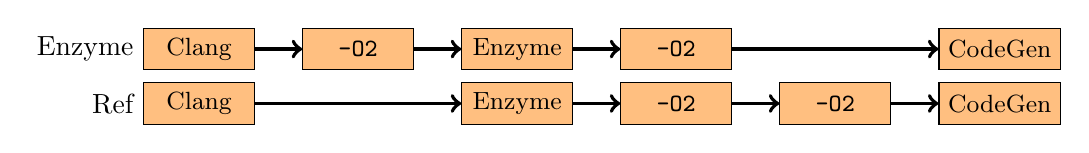
\begin{tikzpicture}[auto, node distance=.15cm and 0.6cm]

    \node [process, label=left:{Enzyme}] (clang1) {Clang};

    \node [process, right= of clang1] (opt1) {\texttt{-O2}};

    \node [process, right= of opt1] (enzyme1) {Enzyme};

    \node [process, right= of enzyme1] (popt1) {\texttt{-O2}};

    
    \node [process, label=left:{Ref}, below= of clang1] (clang2) {Clang};

    \node [process, below= of enzyme1] (enzyme2) {Enzyme};

    \node [process, right= of enzyme2] (opt2) {\texttt{-O2}};

    \node [process, right= of opt2] (popt2) {\texttt{-O2}};

    \node [process, right= of popt2] (cg2) {CodeGen};

    \node [process, above= of cg2] (cg1) {CodeGen};

    \draw [->, line width=0.5mm] (clang1) -- node {} (opt1);
    \draw [->, line width=0.5mm] (opt1) -- node {} (enzyme1);
    \draw [->, line width=0.5mm] (enzyme1) -- node {} (popt1);
    \draw [->, line width=0.5mm] (popt1) -- node {} (cg1);

    \draw [->, line width=0.5mm] (clang2) -- node {} (enzyme2);
    \draw [->, line width=0.5mm] (enzyme2) -- node {} (opt2);
    \draw [->, line width=0.5mm] (opt2) -- node {} (popt2);
    \draw [->, line width=0.5mm] (popt2) -- node {} (cg2);
  \end{tikzpicture}

\caption{The evaluation pipelines.}
  \label{fig:pipeline}
\end{figure}

We evaluate the Enzyme approach by measuring the runtime of seven benchmarks. These benchmarks include the three reverse-mode benchmarks from Microsoft's machine-learning focused ADBench suite: bundle analysis (BA), a long short term memory model (LSTM), and a gaussian mixture model (GMM). We also differentiate two integrators (Euler, RK4) from the Odeint header-only ODE solver library \cite{ahnert2011odeint}; a simple Fast Fourier Fransform (FFT); and a mesh-simulation of the Brusselator chemical dynamics (Bruss) \cite{feinberg1987chemical} recently explored in the context of Neural Differential Equations\cite{rackauckas2020universal}.

\todo{why we chose what we chose.}

\begin{figure}
    \centering

\begin{tabular}{cc}
\hspace*{-1cm}
\begin{minipage}[T]{0.69\linewidth}
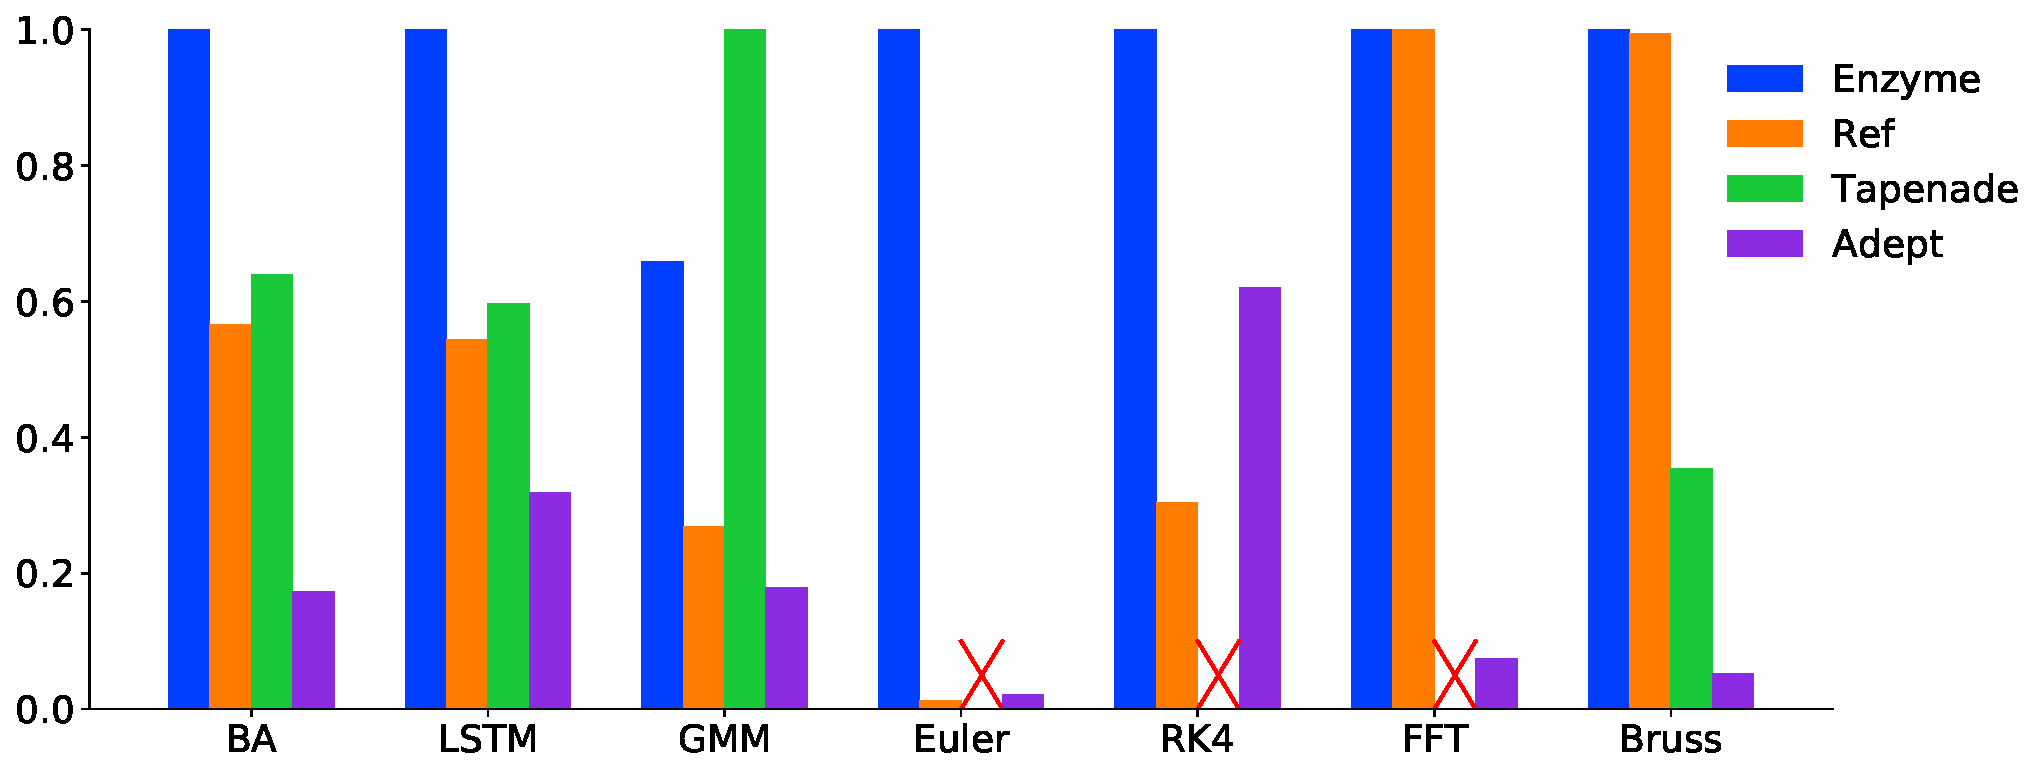
\includegraphics[width=0.99\linewidth]{figs/all.pdf}
\end{minipage}
&
\begin{minipage}[T]{0.29\linewidth}
\hspace*{-1cm} {\scriptsize \begin{tabular}{r|c|c|c|c}
& Enzyme& Ref& Tapenade& Adept\\
BA& \textbf{0.250}& 0.442& 0.391& 1.447\\
LSTM& \textbf{2.405}& 4.426& 4.026& 7.540\\
GMM& 0.261& 0.482& \textbf{0.130}& 0.725\\
Euler& \textbf{0.185}& 14.258& N/A& 8.650\\
RK4& \textbf{3.929}& 12.904& N/A& 6.335\\
FFT& \textbf{0.182}& \textbf{0.182}& N/A& 2.439\\
Bruss& \textbf{0.182}& 0.183& 0.514& 3.444\\
\end{tabular}}
\end{minipage}
\end{tabular}
    \caption{\textbf{\textit{Left:}} Relative speedup of AD systems on the benchmark suite. A red X denotes programs that an AD system does not produce a correct gradient (after accounting for the Tapenade corrections present in ADBench). For each benchmark, we take the geometric mean of the runtime for all test cases, normalizing to the victor. A value of 1.0 denotes the fastest AD system tested for that benchmark, whereas a value of 0.5 denotes that an AD system produced a gradient which took twice as long. \textbf{\textit{Right:}} table with geometric mean runtime in seconds. N/A indicates a benchmark did not work with that system, perhaps producing incorrect results.}
    \label{fig:eval}
\end{figure}

Specifically, to evaluate the effectiveness of AD on optimized IR, we construct two pipelines shown in Figure \ref{fig:pipeline}. The Enzyme pipeline consists of running optimizations before Enzyme's AD, followed by a second round of optimizations. The Reference (Ref) pipeline is identical to the Enzyme pipeline, except that AD is performed before the first round of optimization. This allows us to effectively evaluate the importance of optimization on AD without considering additional confounding factors (such as differing tape implementations) between Enzyme and existing source AD systems. We ran our experiments on a ``quiesced'' AWS c4.8xlarge instance with 60 GiB of memory and 18 cores. To minimize variance, we disabled hyperthreading and Turbo Boost. Taking the geometric mean across all benchmarks, we find that Enzyme outperforms Reference by a factor of is 2.851.

We also compare against the two fastest C/C++ AD tools evaluated in ADBench. These results are presented in Figure \ref{fig:eval}. Enzyme demonstrate superior performance for 7 of the 8 benchmarks. Furthermore the reference pipeline achieves similar performance to Tapenade on the BA and LSTM benchmarks, suggesting that Enzyme's advantage stems from running optimizations first. Tapenade's superior performance on GMM and Enzyme's superior performance on Bruss, however, can be explained by differences in how Enzyme and Tapenade implement their tape structures. Initial optimization also makes a significant impact on the Euler and RK4 tests, explaining much of the performance gap between Enzyme and Adept, whereas Enzyme's more efficient tape structure explains its superior performance on FFT.
\section{Conclusion}
\label{sec:conclusion}
Enzyme demonstrates that it is feasible to perform efficient AD on low-level programs, opening up the door for generic language-independent AD and AD after optimization. This transforms the existing workflow machine learning researchers use to bring ML to foreign code. Instead of rewriting foreign code for machine learning, they can automatically synthesize fast gradients! This opens up the door to apply machine learning to a vast array of new use cases without the substantial effort that a rewrite or new DSL requires.

\paragraph{Broader Impact}
By reducing the amount of work necessary to apply ML to new domains, Enzyme has a generally positive impact. This advances various scientific problem domains with all the positives and negatives that come with it.

\paragraph{Future Work}
Building Enzyme as part of the LLVM compiler infrastructure opens the door for many avenues for future research. Being written as part of a framework for writing optimization, it would be interesting to explore AD-specific optimizations that might not otherwise be handled by a general optimizer. Further, one could apply one of LLVM's existing GPU or parallel code generator  on programs generated by Enzyme~\cite{grosser2011polly, gysi2020domain}. As LLVM can represent GPU~\cite{rhodin2010ptx, holewinski2011ptx} and CPU-parallel programs~\cite{tapir, doerfert2018compiler}, one could extend Enzyme to create gradients for parallel programs. One could also explore the graph problem of determine whether a value should be cached or recomputed beyond a simple heuristic. Enzyme could also be extended to support forward-mode AD, checkpointing, and mixed-mode AD~\cite{mmarxiv}. As shown by the Julia work, Enzyme opens up opportunities for cross-language AD. We would also love to work with the community to assist in porting various physics engines or other codebases to machine learning frameworks.


 
 %efficiently bring new tools 


% \todo{In order to provide a balanced perspective, authors are required to include a statement of the potential broader impact of their work, including its ethical aspects and future societal consequences. Authors should take care to discuss both positive and negative outcomes}
\begin{ack}
Use unnumbered first level headings for the acknowledgments. All acknowledgments
go at the end of the paper before the list of references. Moreover, you are required to declare 
funding (financial activities supporting the submitted work) and competing interests (related financial activities outside the submitted work). 
More information about this disclosure can be found at: \url{https://neurips.cc/Conferences/2020/PaperInformation/FundingDisclosure}.


Do {\bf not} include this section in the anonymized submission, only in the final paper. You can use the \texttt{ack} environment provided in the style file to autmoatically hide this section in the anonymized submission.
\end{ack}

\bibliographystyle{plain}
\bibliography{allpapers}

\end{document}